\label{ch:detector}
\chapter{LHC}
The Large Hadron Collider (LHC) is the highest-energy particle collider in the world. It was designed to expand the frontier of high energy particle collisions in energy and luminosity. This enables LHC experiments to test the Standard Model and search for new physics at higher energies than tested with previous colliders. Collisions at higher energies not only produce more massive particles but also more weakly interacting particles. Fig ~\ref{fig:xs_scaling} shows production cross sections for various processes at hadron colliders. The rate for electroweak physics processes including $W$ and $Z$ scale with the center-of-momentum energy, $\sqrt{s}$.

The LHC consists of a 26.7 km (17 miles) ring, approximately 100 m underground, outside Geneva, Switzerland. Counter-circulating proton (and occasionally heavy ions) beams collide inside four experiments along the beam line: ATLAS, CMS, LHCb, ALICE. ATLAS and CMS are general purpose detectors designed to explore the high energy frontier. LHCb is designed to study the physics of $b$-quarks. ALICE specializes in studying heavy ion collisions. 


\begin{figure}[h!]
  \centering
  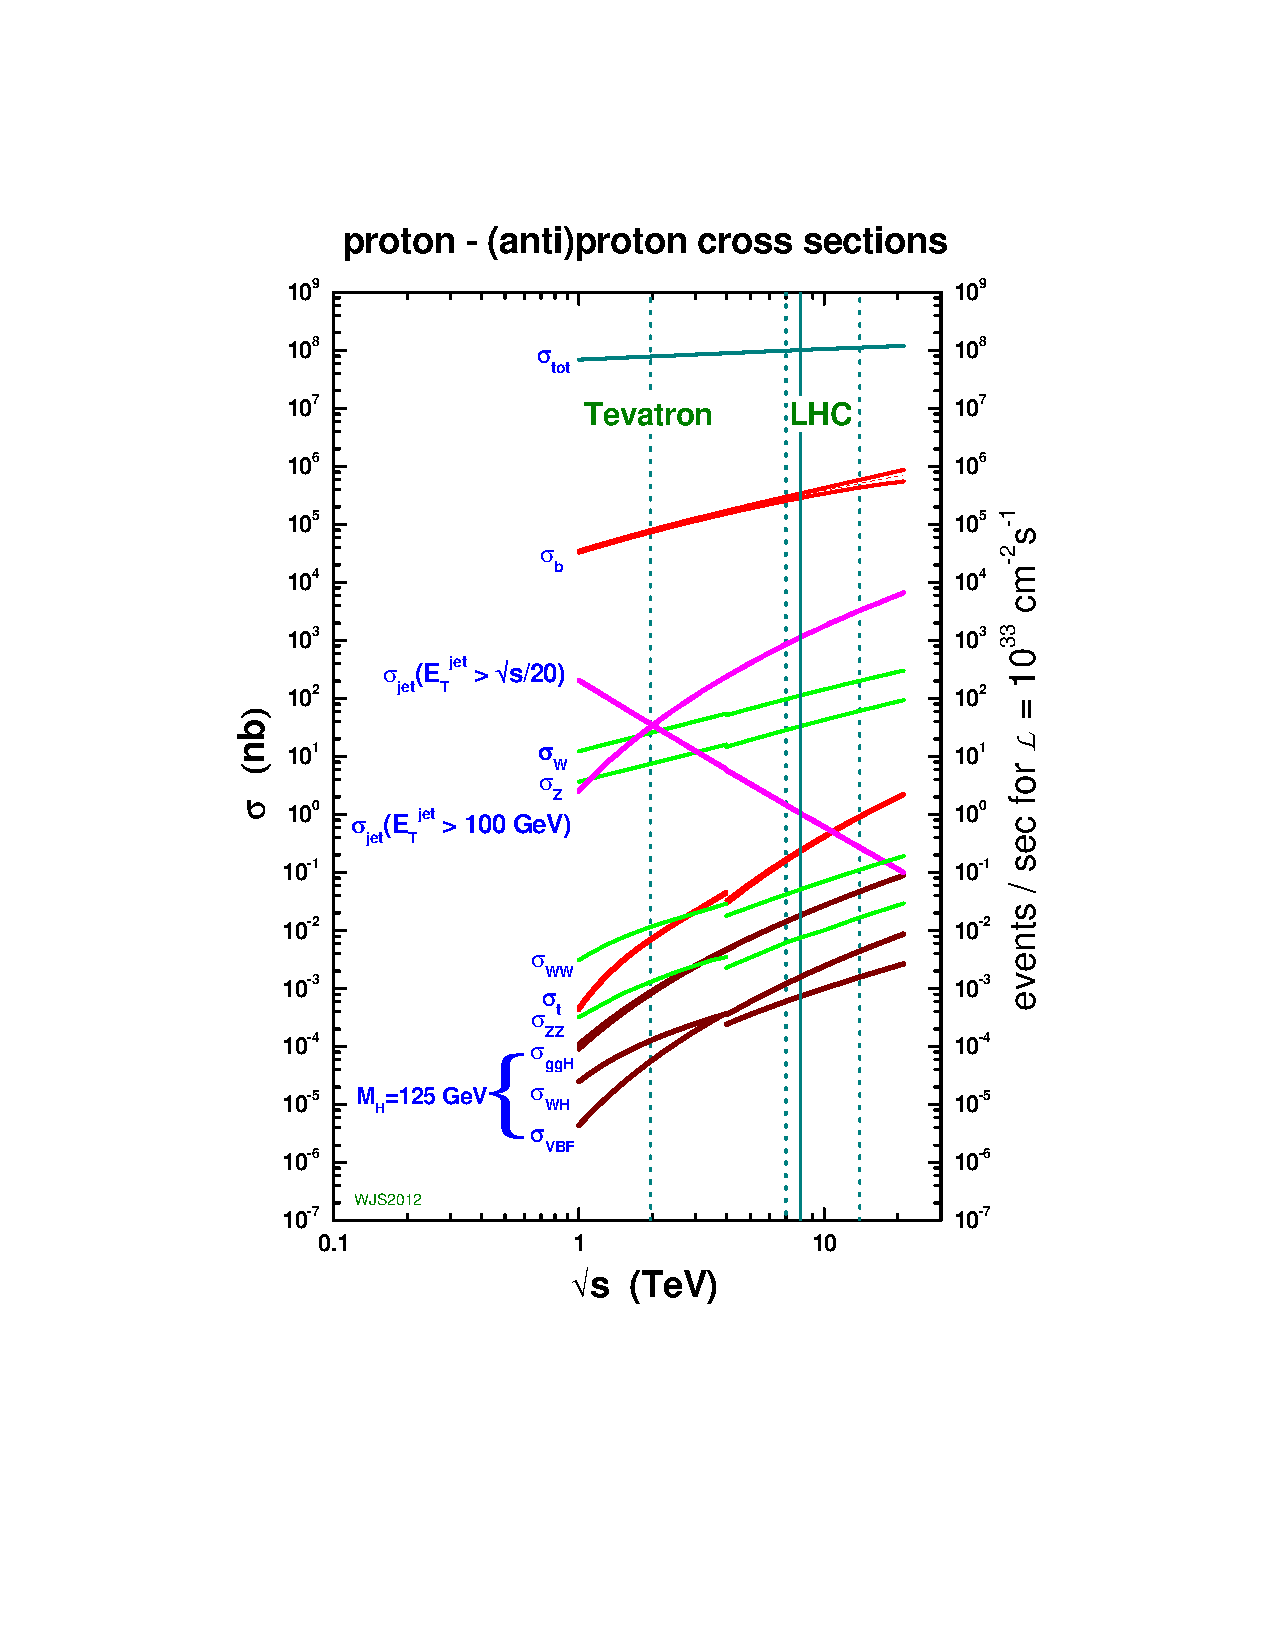
\includegraphics[width=\hsize]{figures/Detector/xs_scaling.pdf}
  \caption{Scaling of cross sections with $\sqrt{s}$. Natasha: write more here}. 
  \label{fig:xs_scaling}
\end{figure}
\FloatBarrier


The first proton beams circulated in September, 2008. Nine days later an electrical fault lead to mechanical damage and liquid helium leaks in the collider. This incident delayed further operation until November 2009, when the LHC became the world's highest energy particle collider, at 1.18TeV per beam. This first operational run continued until 2013, reaching 7 and 8 TeV collision energies. During this run a particle with properties consistent with the Standard Model Higgs boson was discovered. The next run began after a two year shutdown after upgrades to the LHC and experiments. This run lasted from 2013 to 2018 reaching 13 TeV collision energies. This analysis uses data from the second operational run. 
\section{LHC Layout and Design}
The layout of the LHC is shown in Figure ~\ref{fig:lhc_layout}. The red and blue lines in the figure represent the counter-circulating proton beams. The LHC is divided into eight octants.  Octant 4 contains the RF cavities that accelerate the protons and octant 6 contains the beam dump system. Octants 3 and 7 house the collimation systems for beam cleaning. The beams collide inside the four aforementioned experiments. Each octant contains a curved and straight section. The LHC magnets are built with NBTi superconductors cooled with super-fluid Helium to 2K, creating a 8.3T magnetic field to bend the proton beams.


\begin{figure}[h!]
  \centering
  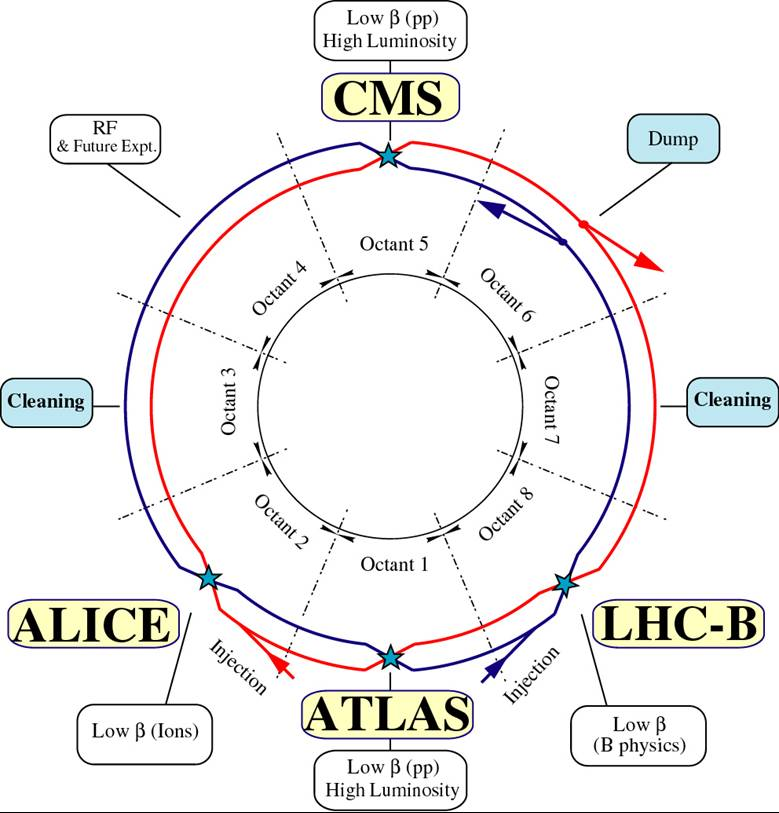
\includegraphics[width=\hsize]{figures/Detector/lhc.jpg}
  \caption{LHC Layout. Natasha write more}. 
  \label{fig:lhc_layout}
\end{figure}
\FloatBarrier


Four sequential particle accelerators are used to accelerate protons from rest as shown in Figure \ref{fig:lhc_accel}. First, Hydrogen gas is ionized to produce protons which are then accelerated to 50 MeV using Linac 2, a linear accelerator. The resulting proton beam is then passed to three circular particle accelerators: Proton Synchrotron Booster, Proton Synchrotron, and Super Proton Synchrotron (SPS), accelerating protons to 1.4, 25, and 450 GeV, respectively. Once the protons exit the SPS, they are injected into the LHC at octant 2 and 8. Each proton bunch contains $\sim 10^{11}$ protons. The spacing between bunches is 25 ns, which means each beam contains 3564 bunches. However, some bunches are left empty due to injection and safety requirements, yielding 2808 bunches per beam. Once the proton beams are injected they are accelerated to 13 TeV. 


\begin{figure}[h!]
  \centering
  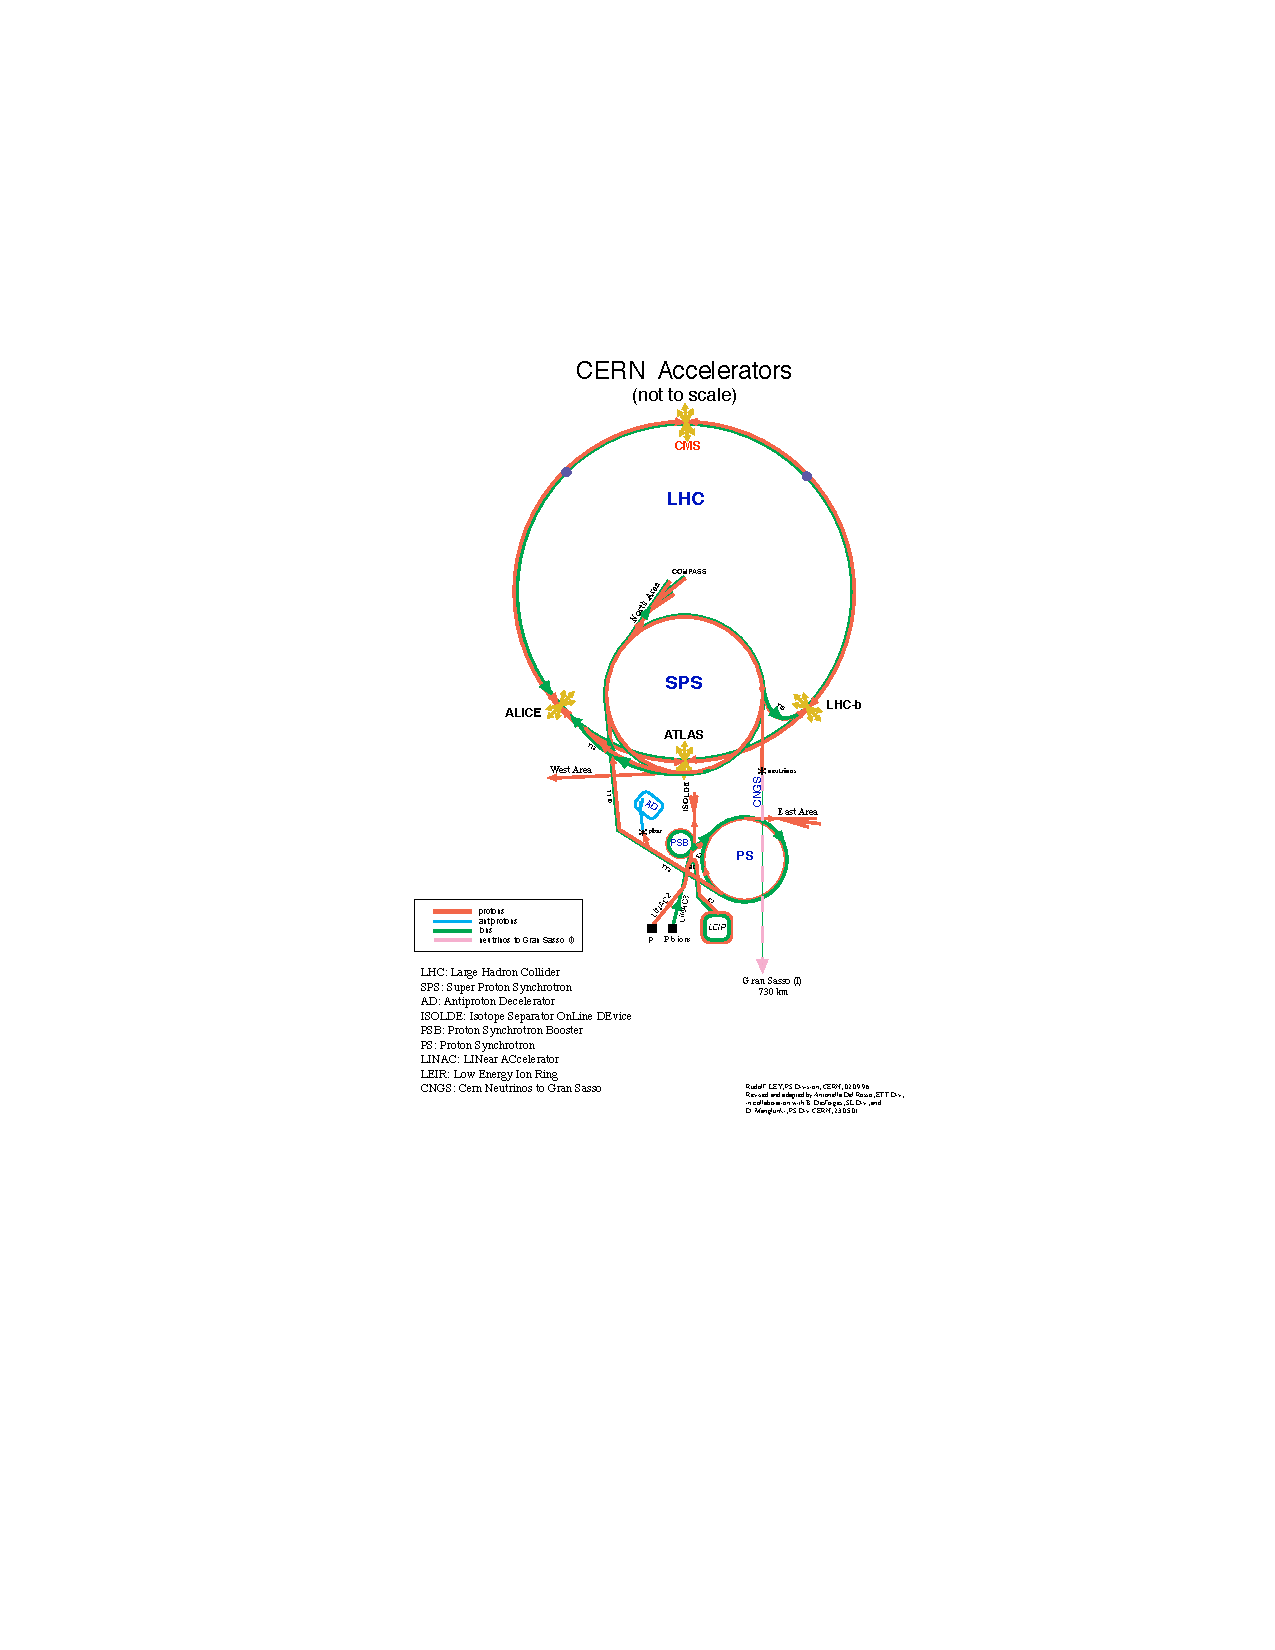
\includegraphics[width=\hsize]{figures/Detector/lhc_accel.pdf}
  \caption{LHC Accelerator. Natasha write more}. 
  \label{fig:lhc_accel}
\end{figure}
\FloatBarrier


As many new physics models predict cross-sections below the weak scale it was important to design the LHC to be capable of collecting enough data, by running in high luminosity conditions. The machine luminosity depends only on beam parameters:

\begin{equation}
L=\frac{N_{p}^{2}f}{4\epsilon\beta^{*}}F
\end{equation}

where $N_{p}$ is the number of protons per bunch, f is the bunch crossing frequency, $\epsilon$ is the transverse beam emittance, $\beta^{*}$ is the amplitude function at the collision point, and F is the geometric luminosity reduction factor due to the beams crossing at an angle (rather than head-on). 

\chapter{The ATLAS Detector}
The ATLAS detector measures the position, momentum and energy of particles produced in the proton collisions by using magnetic fields, silicon detectors, sampling calorimeters, and gaseous wire detectors. It is located approximately 100 m underground at Point-1 around the LHC beam line and weighs 7000 metric tons. The detector is 46 m long, 25 m high, 25 m wide  as shown in Figure \ref{fig:atlas_detectors}. The detector can be divided into three subsystems: the Inner Detector (ID), the Calorimeters, and the Muon Spectrometer (MS). Figure \ref{fig:particle_detection} shows an overview of how different particles interact in the detector.
\begin{figure}[h!]
  \centering
  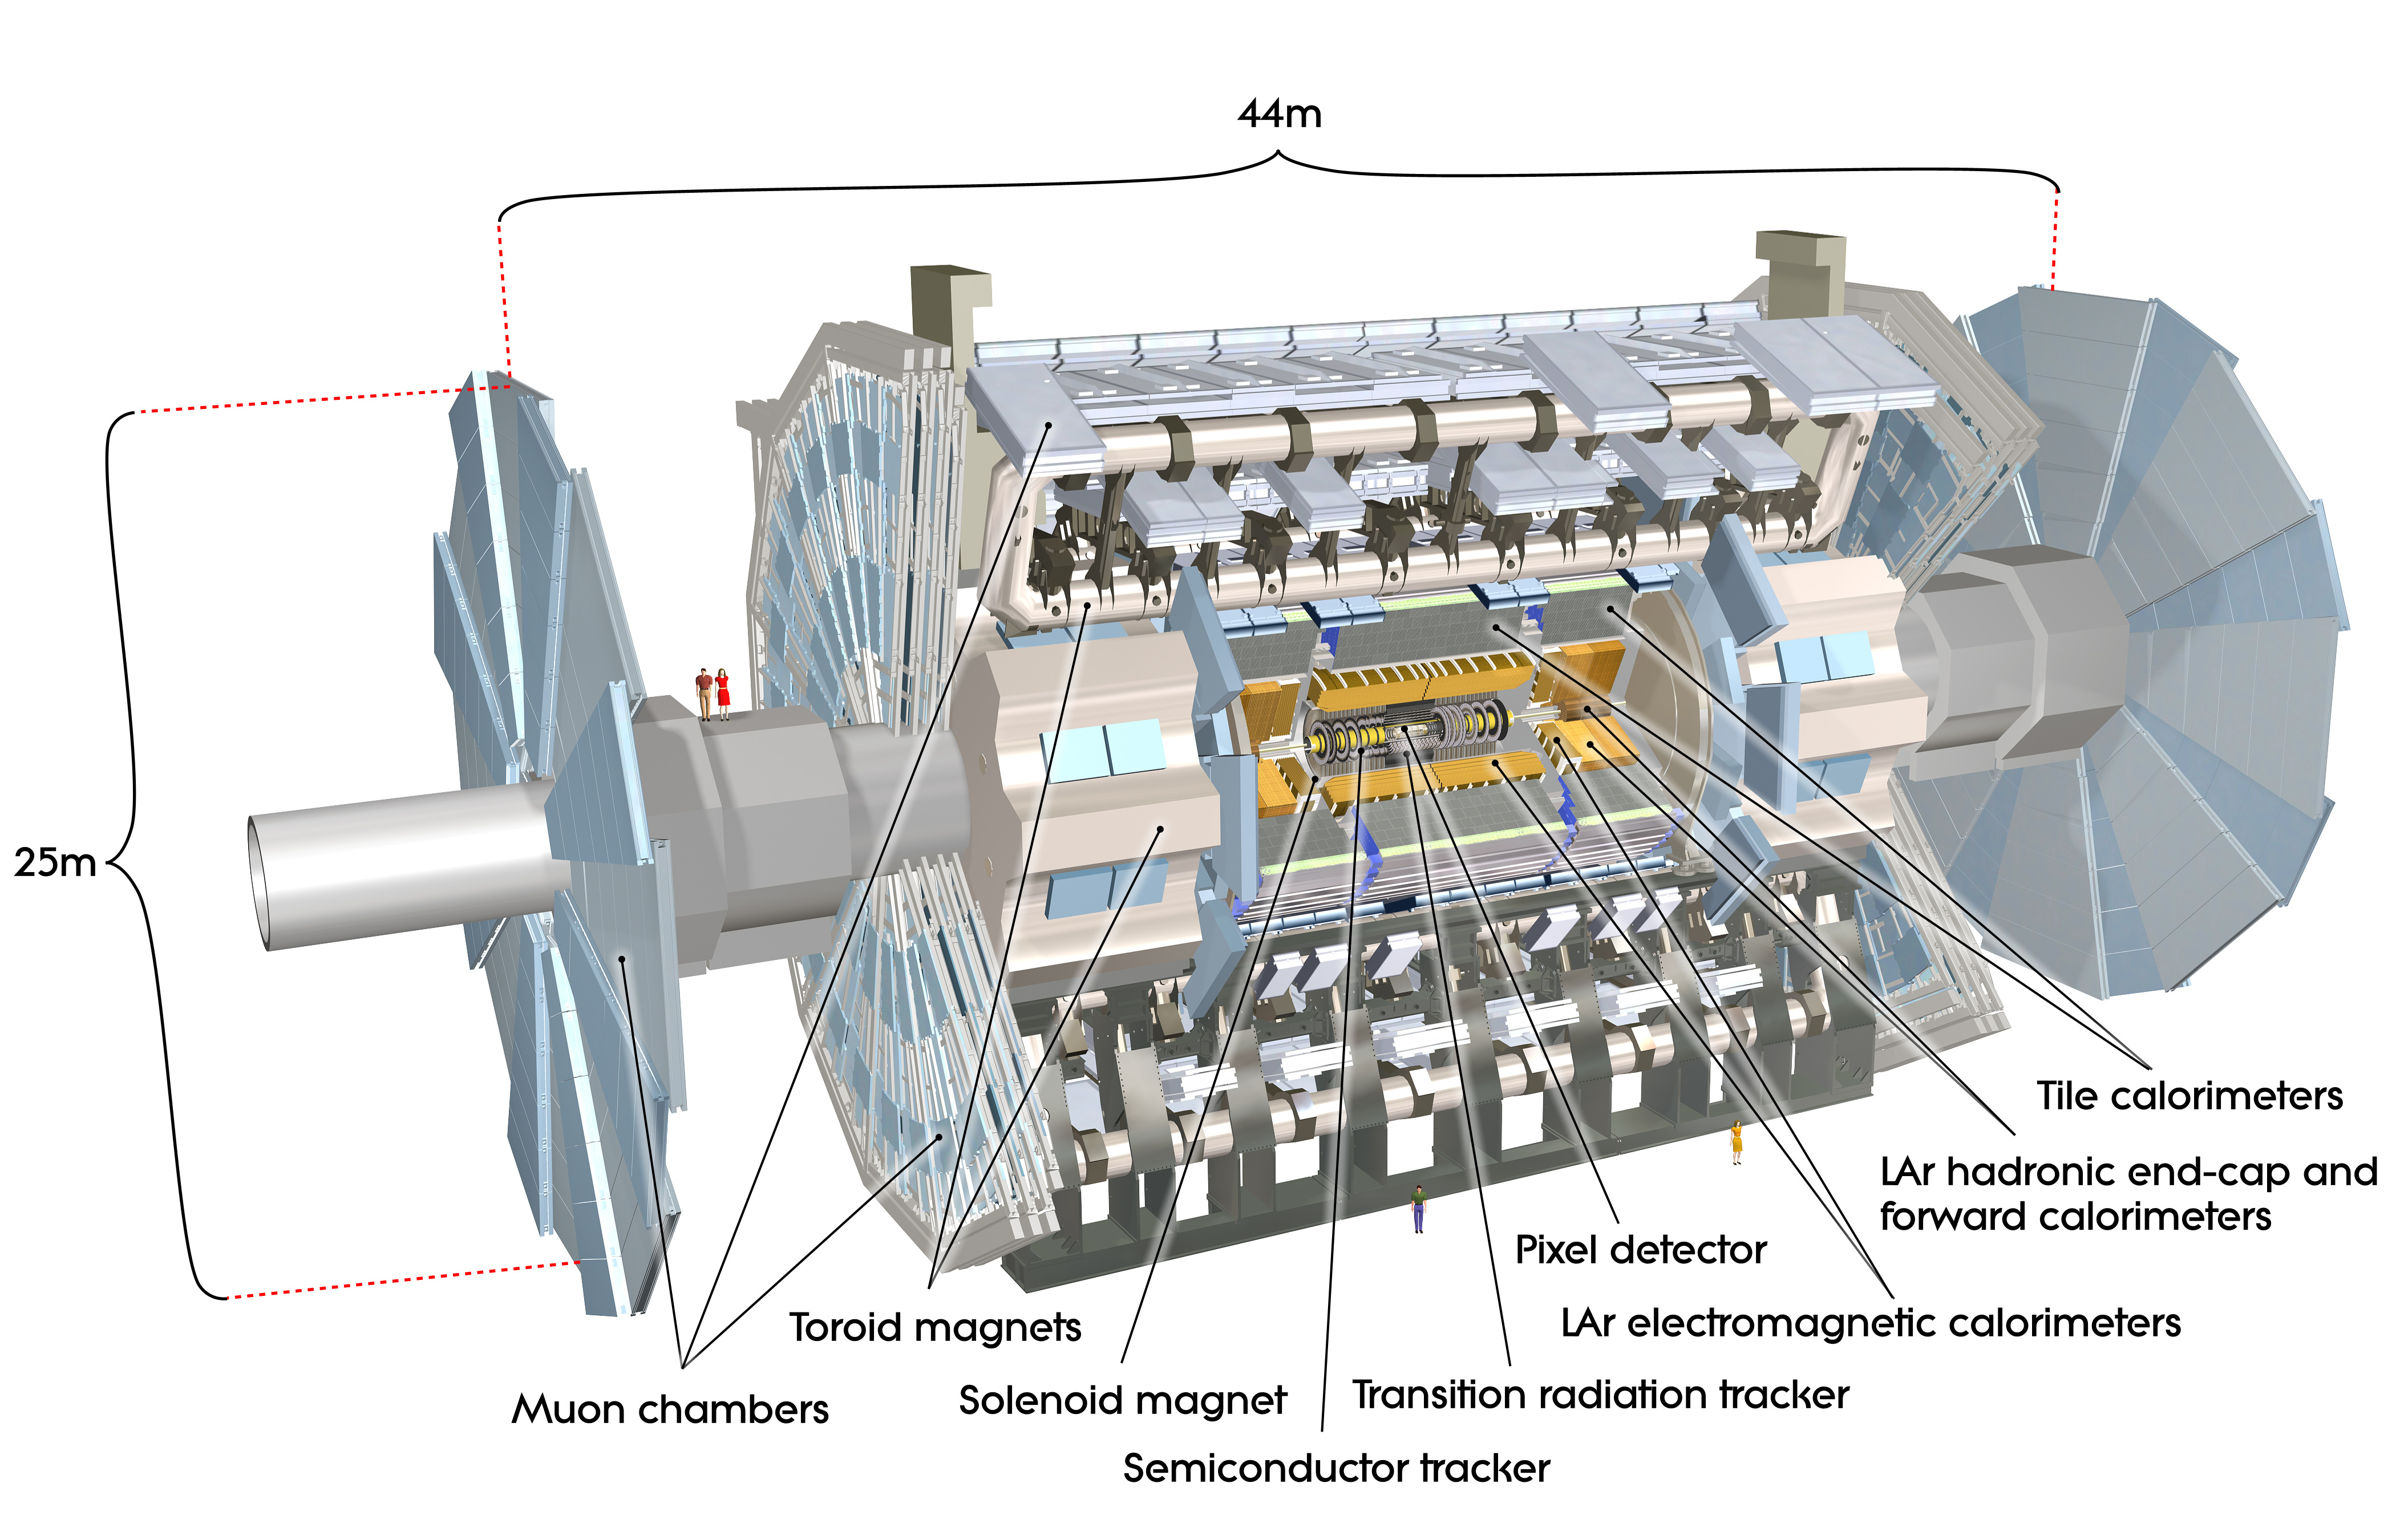
\includegraphics[width=\hsize]{figures/Detector/atlas.jpg}
  \caption{Big picture layout of ATLAS detector. Natasha: write more} 
  \label{fig:atlas_detectors}
\end{figure}
\FloatBarrier

\begin{figure}[h!]
  \centering
  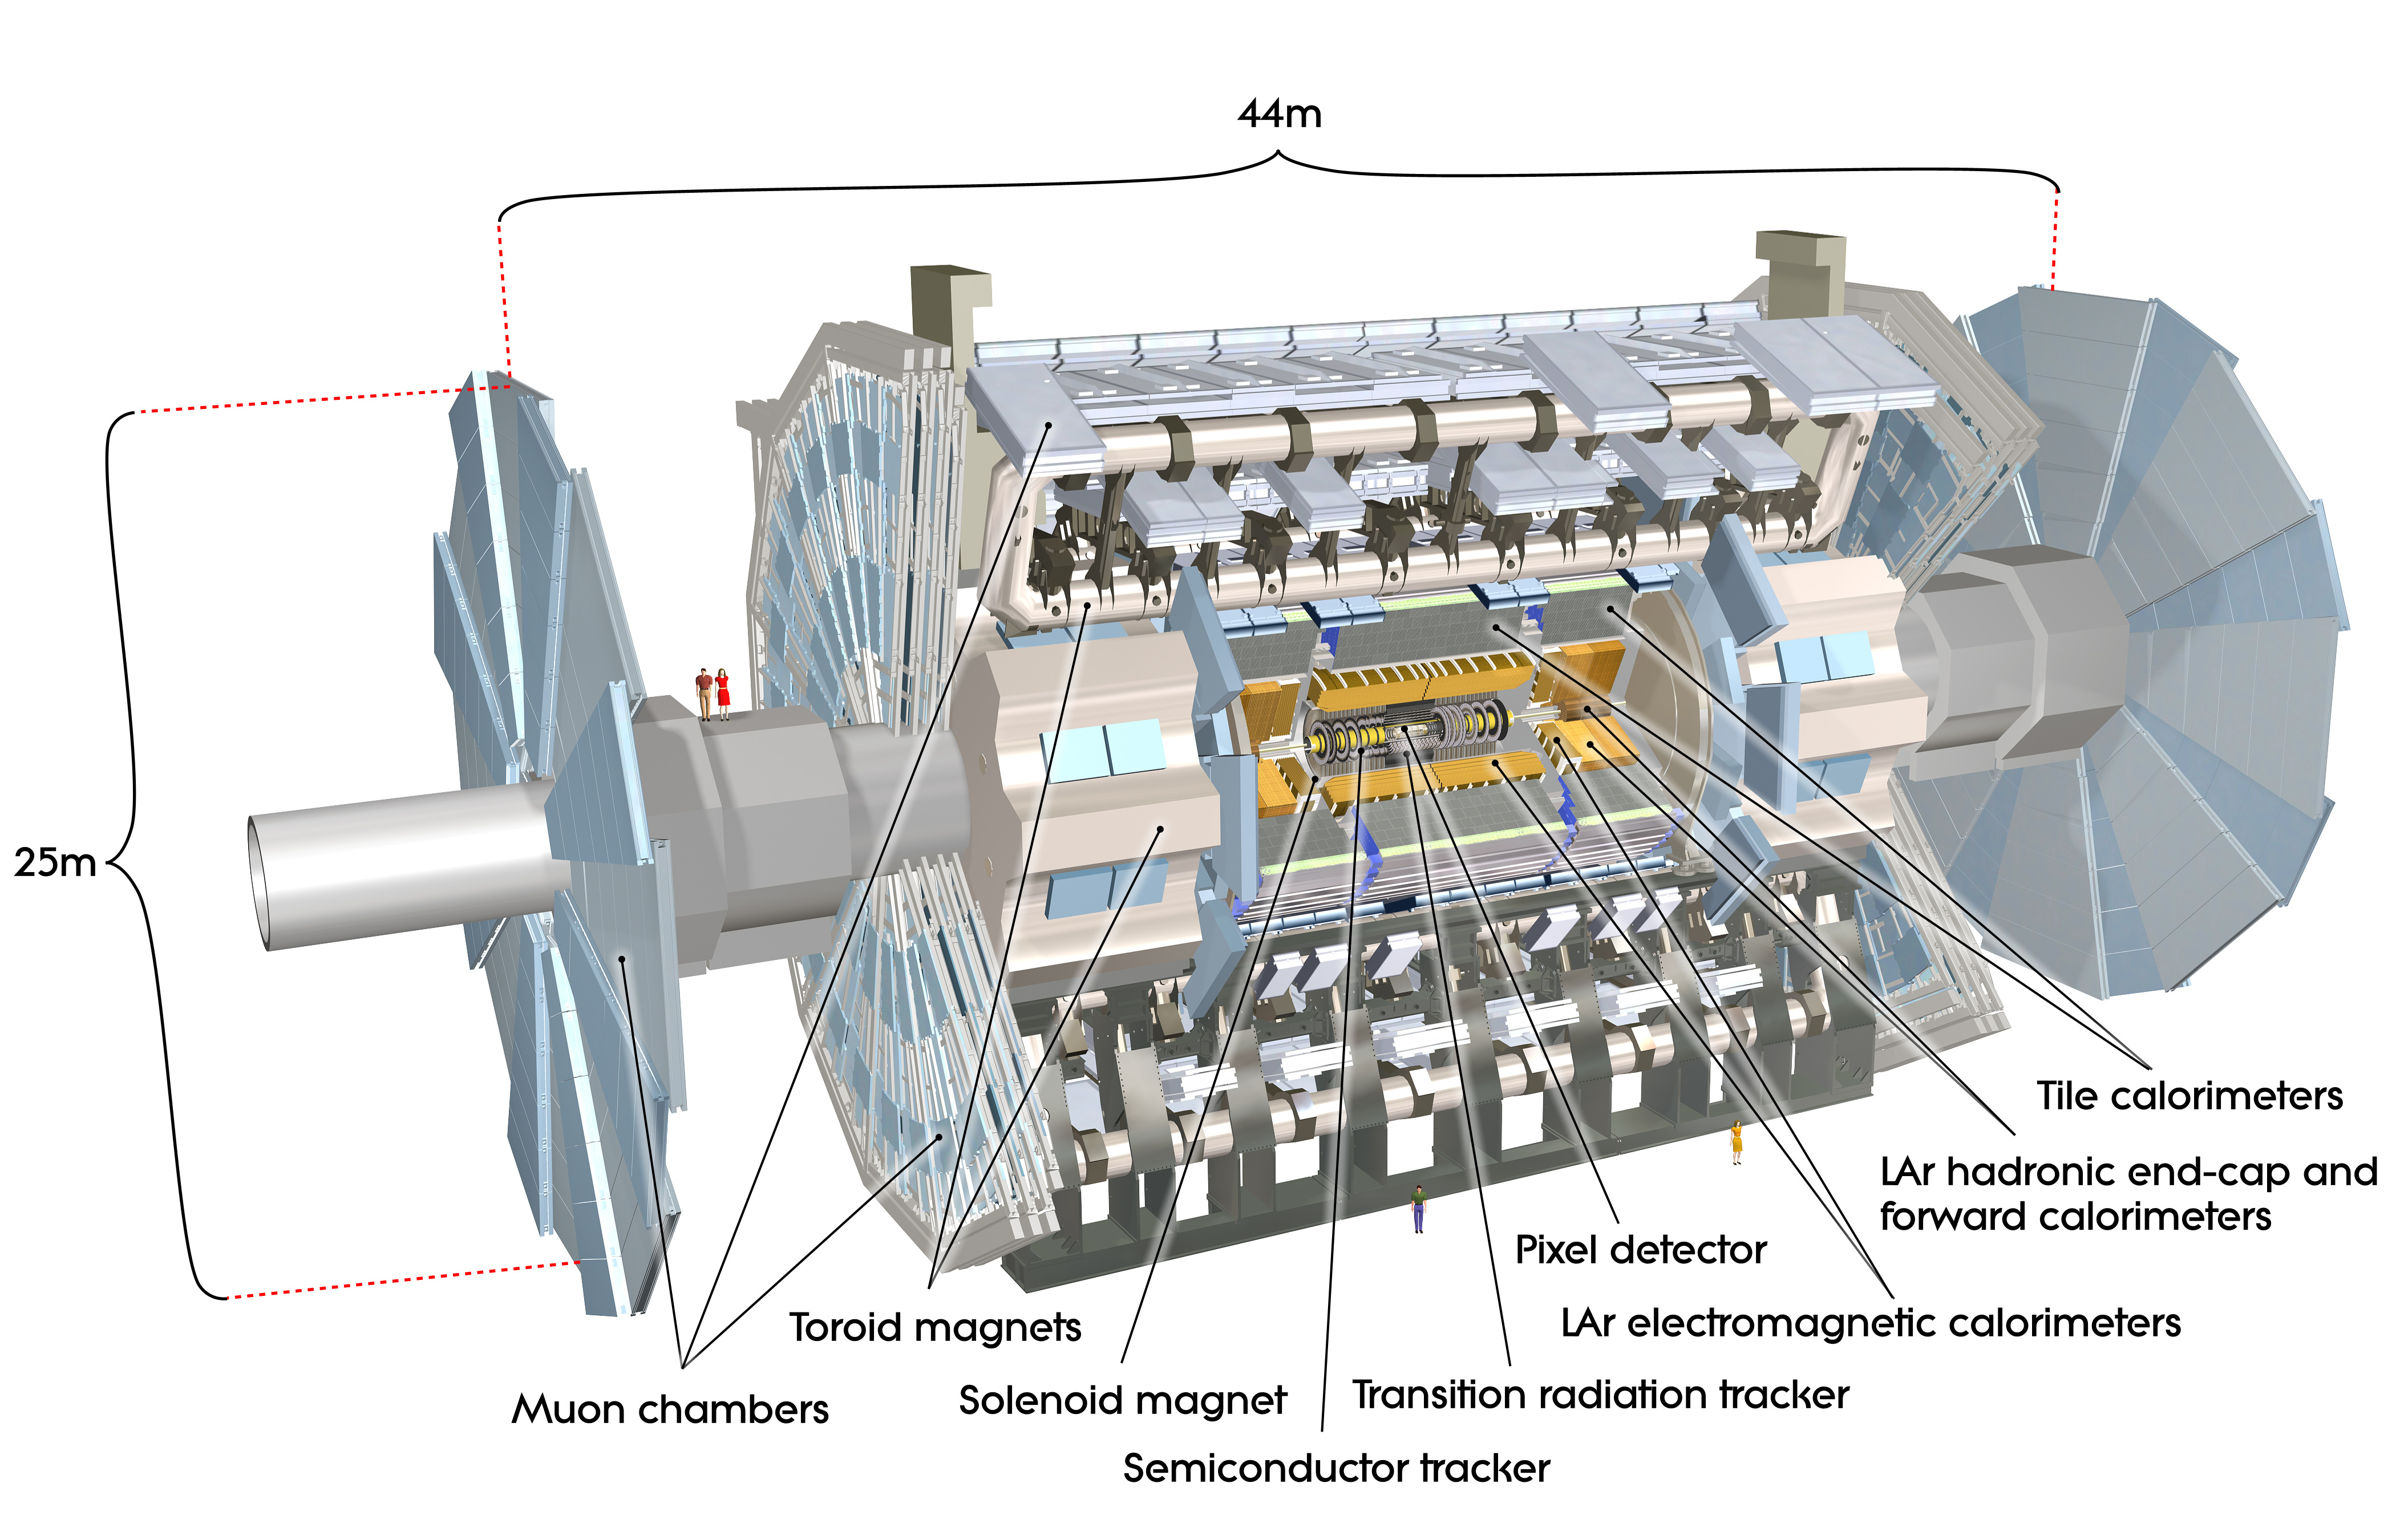
\includegraphics[width=\hsize]{figures/Detector/atlas.jpg}
  \caption{Big picture layout of ATLAS detector. Natasha: write more} 
  \label{fig:atlas_detectors}
\end{figure}
\FloatBarrier

\begin{figure}[h!]
  \centering
  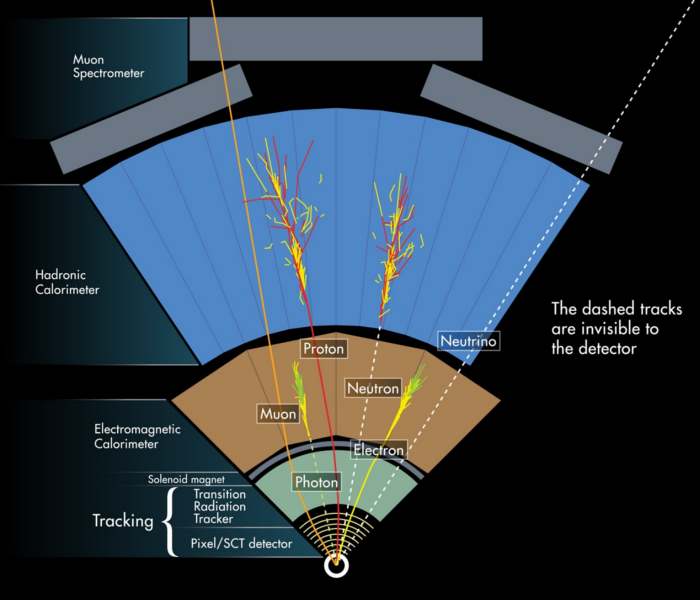
\includegraphics[width=\hsize]{figures/Detector/particle_detection_atlas.png}
  \caption{A simplified schematic of how different particles interact and are detected within ATLAS.} 
  \label{fig:particle_detection}
\end{figure}
\FloatBarrier

\section{Coordinate System}
The trajectory of particles within ATLAS is measured relative to the nominal interaction point. The z-axis points along the beam line, such that when the LHC is viewed from above, the counter-clockwise circulating beam points along the positive-$z$ direction. The $x-y$ plane is transverse to the beam line, with the positive x-axis pointing towards the center of the LHC ring. The positive $y$-axis points vertically upward. The azimuthal angle, $\phi$, is the angular distance about the $z$-axis, with $\phi=0$ along the $x$-axis. The polar angle from the $z$-axis is denoted as $\theta$.  However, this quantity is not Lorentz invariant, like rapidity, $y=\frac{1}{2}\ln\frac{E+p_{z}}{E-p_{z}}$, where $E$ is the energy of the particle considered, and $p_{z}$, is it's momentum along the $z$-axis. Pseudo-rapidity is preferred as $\Delta \eta$ is invariant under boosts along $z$ and particle production is approximately invariant under $\eta$. For massless particles, rapidity and a related quantity, pseudorapidity, are the identical. The pseudorapidity is defined as: $\eta = -ln tan(\frac{\theta}{2})$.  This quantity is preferred as it is purely a geometric quantity, independent of particle energy. Angular separation between particles in ATLAS are given by $\Delta R = \sqrt{\Delta \eta^{2}+\Delta \phi^{2}}$. The distance from the beamline is given by $r=\sqrt{x^{2}+y^{2}}$
 
\section{Inner Detector}
The Inner Detector (ID) was designed to identify and reconstruct vertices, distinguish pions from electrons, and measure the momentum of charged particles. The ID uses three different technologies for particle reconstruction: the Pixel Detector, Semiconductor Tracker (SCT), and the Transition Radiation Tracker (TRT), shown in Figure \ref{fig:ID} and \ref{fig:barrelID}. The entire ID is immersed in a 2T solenoidal magnetic field parallel to the $+z$-axis, causing charged particles to bend in the transverse-plane, allowing particle momentum measurements. 

\begin{figure}[h!]
  \centering
  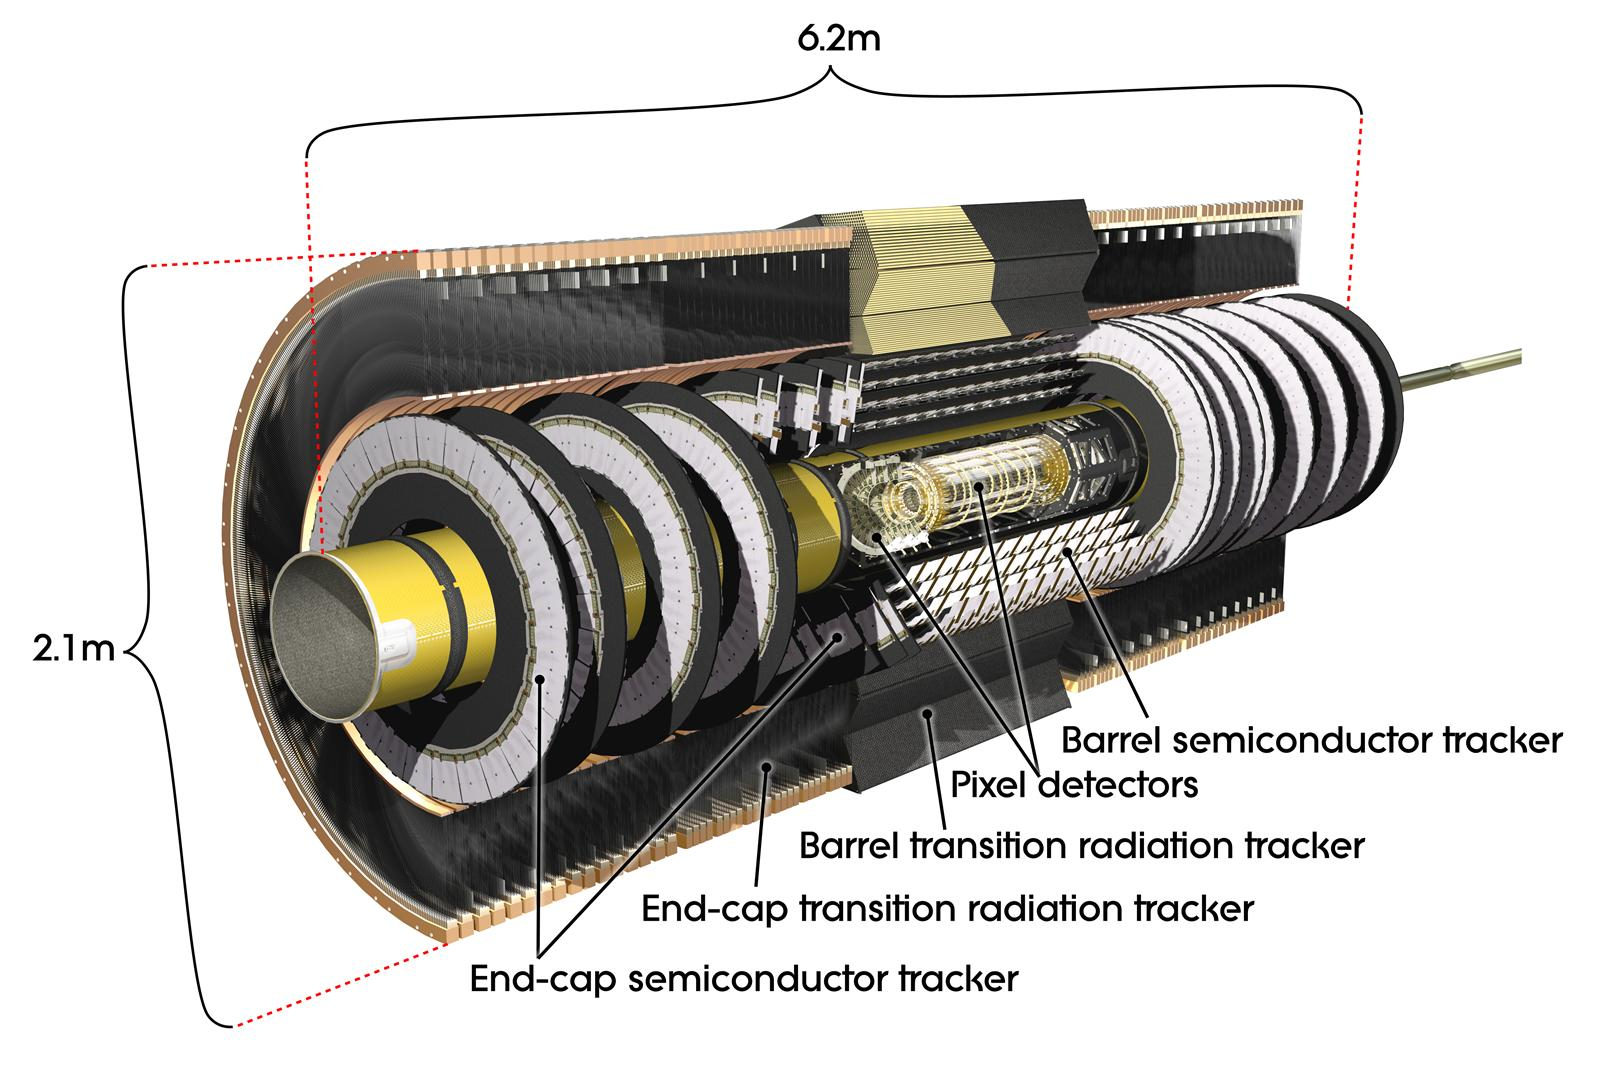
\includegraphics[width=\hsize]{figures/Detector/tracker_layout.jpg}
  \caption{Layout of ATLAS Inner Detector} 
  \label{fig:ID}
\end{figure}
\FloatBarrier


\begin{figure}[h!]
  \centering
  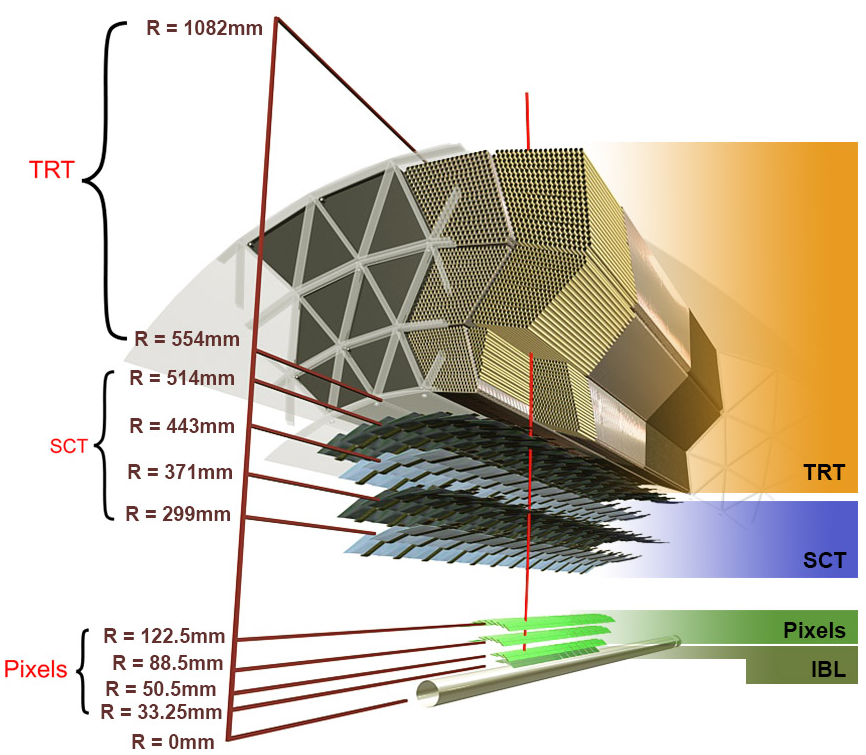
\includegraphics[width=\hsize]{figures/Detector/tracker_barrel.png}
  \caption{Layout of ATLAS ID Barrel System.} 
  \label{fig:barrelID}
\end{figure}
\FloatBarrier


\subsection{Pixel Detector}
The pixel detector consists of four barrel layers between r = 32.7 and 122.5 mm, extending to $|z|=400.5 $mm. The remaining detectors are arranged in barrels and forward and backward rings. The innermost pixel barrel, the Insertable b-Layer (IBL), only extends to $|z|=332$ mm. The pixel detectors closer to the beam line (larger $\eta$ values) consists of six parallel cylindrical rings of pixel detectors transverse to the beam line. The entire pixel detector consists of 1744 identical pixel sensors each with 46080 readout channels, totaling about 80 million individual pixels. Most of the pixel sensors are $50\times400\mu m^{2}$.  Each pixel has a position resolution of 14$\mu$m in $\phi$ and 115 $\mu$m in the $z$ direction.
\subsection{Semiconductor Tracker}
The SCT is located outside the pixel detector and has the same barrel and endcap geometry as the pixel detector. SCT sensors are 80$\mu$m $\times$ 12 cm with a 80$\mu$m strip pitch. In the barrel the strips are parallel to the $z$-axis and are segmented in $\phi$. In the endcaps, the strips extend radially. Sensors are grouped in modules containing two layers of strips rotated 40 mrad with respect to each other. This offset allows for the two-dimensional position of a track to be determined by identifying the crossing point of the strips that registered a hit. SCT modules measure tracks with an accuracy of 17 $\mu$m in $r-\phi$ and 580$\mu$m in $z(r)$ in the barrel (end-cap) region.
\subsection{Transition Radiation Tracker}
The transition radiation tracker (TRT), enveloping the SCT, is a gaseous straw-tube tracker mainly used for electron/pion track separation. Each straw is 4 mm in diameter and filled with a Xe-C$O_{2}$-$O_{2}$ gas mixture. An anode wire at the center of the straw is held at ground potential, while the walls of the straw are kept at -1.4kV. When a charged particle passing through the TRT ionizes the gaseous mixture, the resulting ions form an avalanche on the anode wire with a gain of $\sim 10^{4}$. The signal from the anode wire is then digitized and discriminated. Signals passing a low threshold cutoff are used to distinguish noise from tracks. Signals passing a high threshold cutoff are sensitive to transition radiation (TR). TR photons are emitted when charged particles pass between materials with different dielectric constants. The probability that a charged particle with energy $E$ and mass $m$ passing between two materials emits a TR photon in the keV range is proportional to $\gamma=E/m$. In the TRT staws these often then convert via the photoelectric effect, causing a large avalanche triggering the high-threshold. Since electrons have a smaller mass than pions, electron tracks are more likely to trigger the high threshold. This then provides discrimination between electrons and charged hadrons.

The barrel region of the TRT extends from $r=$563-1066 mm and $|z| < 712$ mm. Barrel Straws are 144 cm long (divided  $\sim \eta \approx 0$) and orientated parallel to the beam direction. End-cap straws extend radially and are 37 cm long. There are 53,544 straws in the barrel and 160,000 straws in the end-caps. Radiator mats of polypropylene/polyethylene fibers in the barrel are aligned perpendicular to the barrel straws (with holes for the straws to pass through). In the end-cap region, radiator foils are layered between the radial TRT straws. 

The arrival time of the signal pulse is sensitive to the distance between the charged particle track and the anode wire and allows for a hit resolution of 130$\mu$m. The TRT extends to $|\eta| = 2.0$ and provides about 36 hits per track.
\section{Calorimeters}
The ATLAS electromagnetic and hadronic calorimeters (EMC and HCAL, respectively) absorb and measure the energy of high energy hadrons, photons, and electrons with $|\eta| < 4.9$. Both systems use sampling calorimeters which consist of alternating layers of dense absorbing and active layers. In the absorbing layer particles interact and lose energy, creating showers. These showers are then detected and measured in the active layer. The amount of charge measured in the active material scales with the energy of the incident particle, and thus provides a measurement of the particle's energy. An overview of the layout of the calorimeter system is shown in Figure \ref{fig:calo_overview}.

The EMC measures and contains the energy of electromagnetically interacting particles. It consists of layered accordion-shaped Lead absorber plates and electrodes immersed in liquid Argon with 170k channels.. Using accordion-shaped electrode and absorbers ensures $\phi$ symmetry and coverage. The EMC is composed of a barrel part ($|\eta| < 1.475$), two end-caps ($1.375<|\eta| < 3.2$), and a presampler ($|\eta| < 1.8$).  The presampler, containing only liquid Argon, corrects for upstream energy losses of electrons and photons. The EMC barrel is segmented into three layers. The first layer has finest segmentation with readout cells extending $\Delta \eta \times \Delta \phi = 0.025/8 \times 0.1$. This provides a precise shower measurements used to separate prompt photons from $\pi^{0} \rightarrow \gamma \gamma$ decays. The second layer has coarser segmentation and is approximately 16 radiation lengths long. A radiation length is the average distance an electron travels before losing all but 1/$e$ of its energy to bremsstrahlung. The last layer is the most coarse and measures the tail of the electromagnetic shower. A schematic of the ECAL is shown in Figure \ref{fig:ecal}. 

The hadronic calorimeter located outside the EMC and is used to contain and measure the energy of hadronically interacting particles. It consists of a tile calorimeter (TileCal), hadronic end-cap calorimeter (HEC), and liquid Argon forward calorimeter (FCAL). TileCal is located behind the LAr EMC and uses steel absorbers and liquid Argon as the active material. TileCal consists of three barrel layers in the central and forward regions, extending up to $|\eta| < 1.7$. Photons generated from hadronic interactions are collected via wavelength-shifting fibers connected to photomultiplier tubes, as shown in Figure ~\ref{fig:hcal}. The HEC lies behind the EMC endcap wheels. It uses copper absorbers and liquid Argon as the active material and covers $1.5 < |\eta| < 3.2$. Finally, the FCAL covers $3.1 < |\eta| < 4.9$ and consists of three modules all using liquid Argon as the active material. The first module uses copper absorber and was designed for electromagnetic measurements. The second and third modules consist of tungsten absorber and are used to measure the kinematics of hadronically interacting particles. A schematic of the HCAL is shown in Figure \ref{fig:hcal}. 

\begin{figure}[h!]
  \centering
  \includegraphics[width=\hsize]{figures/Detector/calo_overview.pdf}
  \caption{Overview of ATLAS electromagnetic and hadronic calorimeters.} 
  \label{fig:calo_overview}
\end{figure}
\FloatBarrier


\begin{figure}[h!]
  \centering
  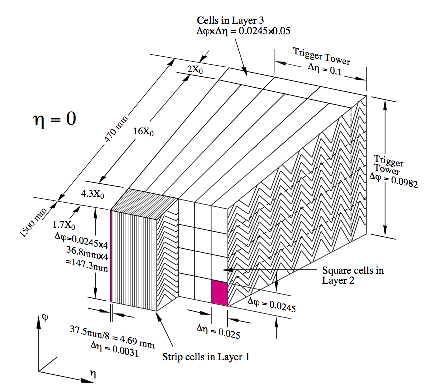
\includegraphics[width=\hsize]{figures/Detector/ecal.pdf}
  \caption{Schematic of ECAL.} 
  \label{fig:ecal}
\end{figure}
\FloatBarrier




\begin{figure}[h!]
  \centering
  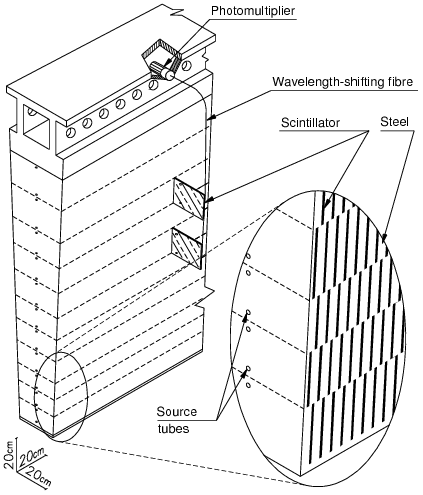
\includegraphics[width=\hsize]{figures/Detector/hcal.png}
  \caption{Schematic of HCAL.} 
  \label{fig:hcal}
\end{figure}
\FloatBarrier


The energy resolution of the calorimeter subsystems are:

$\frac{\sigma_{E}}{E}=\frac{10\%}{\sqrt{E}}\bigoplus 0.7\%$ EMC

$\frac{\sigma_{E}}{E}=\frac{50\%}{\sqrt{E}}\bigoplus 3\%$ hadronic barrel 

$\frac{\sigma_{E}}{E}=\frac{100\%}{\sqrt{E}}\bigoplus 10\%$ hadronic end-cap


\section{Muon Spectrometer}
The muon spectrometer (MS) is the outermost detector system in ATLAS. Muons with a $p_{T}>4$ GeV are energetic enough to reach the MS. To measure the momentum of these muons barrel and end-cap toroid magnets are used covering $|\eta| < 1.4$ and $1.6<|\eta|<2.7$. For $1.4 < |\eta| < 1.6$, a combination of the barrel and end-cap toroidal magnetic fields bend muon trajectories. The detector in the barrel region form three concentric rings at $R=5, 7.5, 10$m and are segmented in $\phi$ to accommodate the magnets. The end-cap region consists of three circular planes perpedicular to $z$ and located at $|z|=7.4, 14, 21.5$m from the interaction region. An additional detector at $|z|=10.8$m covers the transition region between the barrel and end-cap.

The MS readout consists of four subsystems: Monitored Drift Tubes (MDT), Cathode Strip Chambers (CSC), Resistive Plate Chambers (RPC), and Thin Gap Chambers (TGC). The first two subsystems are used primarily for measuring muon track parameters, while the RPC and TGC subsystems are used for muon triggering. A schematic of this system is shown in Figure ~\ref{fig:muonsys}. 

The MDT subsystem consists of precision tracking chambers for $|\eta|<2.7$, except for the inner most end-cap layer ($2.0 < |\eta| < 2.7$), where CSCs are used. The basic unit of MDT chambers are thin walled Aluminum tubes with a diameter of 3 cm and length of 0.9-6.2 m. These tubes are filled with a mixture of Ar-C$O_{2}$ gas with a  50$\mu$m W-Rn wire running down the center of the tube, which is kept at 3080 V. Since the maximum drift time of these chambers is $\sim$ 700 ns, they are not used for triggering. MDT chambers consist of 3-4 layers of tubes mounted on a rectangular support system, as seen in Figure ~\ref{fig:muon_mdt}, orientated along $\phi$ to measure the coordinate in the bending plane of the magnetic field with a resolution of 35 $\mu$m.

The MDT subsystem can only handle hit rates below 150Hz/c$m^{2}$. For this reason, CSCs are used in the innermost end-cap layer where hit rates are larger. CSCs can handle hit rates up to 1000Hz/c$m^{2}$. CSC are multiwire proportional chambers. These chambers are filled with a Ar-C$O_{2}$ gas mixture and evenly spaced wires kept at 1900 V. These wires are orientated in the radial direction but not read out. Instead on one side of the cathode are copper strips parallel to the wires, measuring $\eta$, while on the other side of the cathode are strips parallel to the wires measuring $\phi$. The width between strips is approximately 1.5 mm providing a resolution of 60 $\mu$m in the bending-plane and 5 mm in the non-bending plane. 

Since the CSC and MDT systems do not have prompt timing signals, the RPC and TGC systems are used for triggering. The RPC system is used in the barrel region ($|\eta| < 1.05$). RPC consist of two parallel resistive plates separated by a 2 mm insulated spacer with 100 mm spacing kept at 9.8 kV, as shown in Figure\ref{fig:muon_rpc}. A gaseous mixture of $C_{2}H_{2}F_{4}$, $C_{4}H_{10}$, and $SF_{6}$ fills the space between the two plates. Metallic strips on the outer faces of the plates are used to read out signals produced by the gas ionizing. The middle barrel layer consists of two layers of RPCs on either side of the MDT layer and one layer on the outermost MDT layer. Each layer contains two orthogonal sets of metallic strips providing $\eta$ and $\phi$ measurements. The timing resolution of RPCs is 1.5 ns, and therefore may be used to identify bunch crossings. 

Finally, the TGCs are used in the end-cap regions and are primarily used to provide L1 trigger decisions and $\phi$ measurements. TGCs are multi-wire proportional chambers consisting of arrays of gold-coated tungsten wires placed between two cathode planes. These wires are separated by 1.8 mm and cathodes are 1.4 mm from the wires. Orthogonal to the wires, on the opposite side of the cathode plane are copper strips held at 2900 V. The chambers are filled with a mixture of $CO_{2}$ and n-pentane gas, the latter acts as a quenching gase to prevent avalances initiated by secondary $\gamma$-rays from the primary avalanche. Figure ~\ref{fig:muon_tgc} is a schematic of a TGC. The timing resolution of TGCs is less than 25 ns and therefore they are used for bunch crossing measurements. 

\begin{figure}[h!]
  \centering
  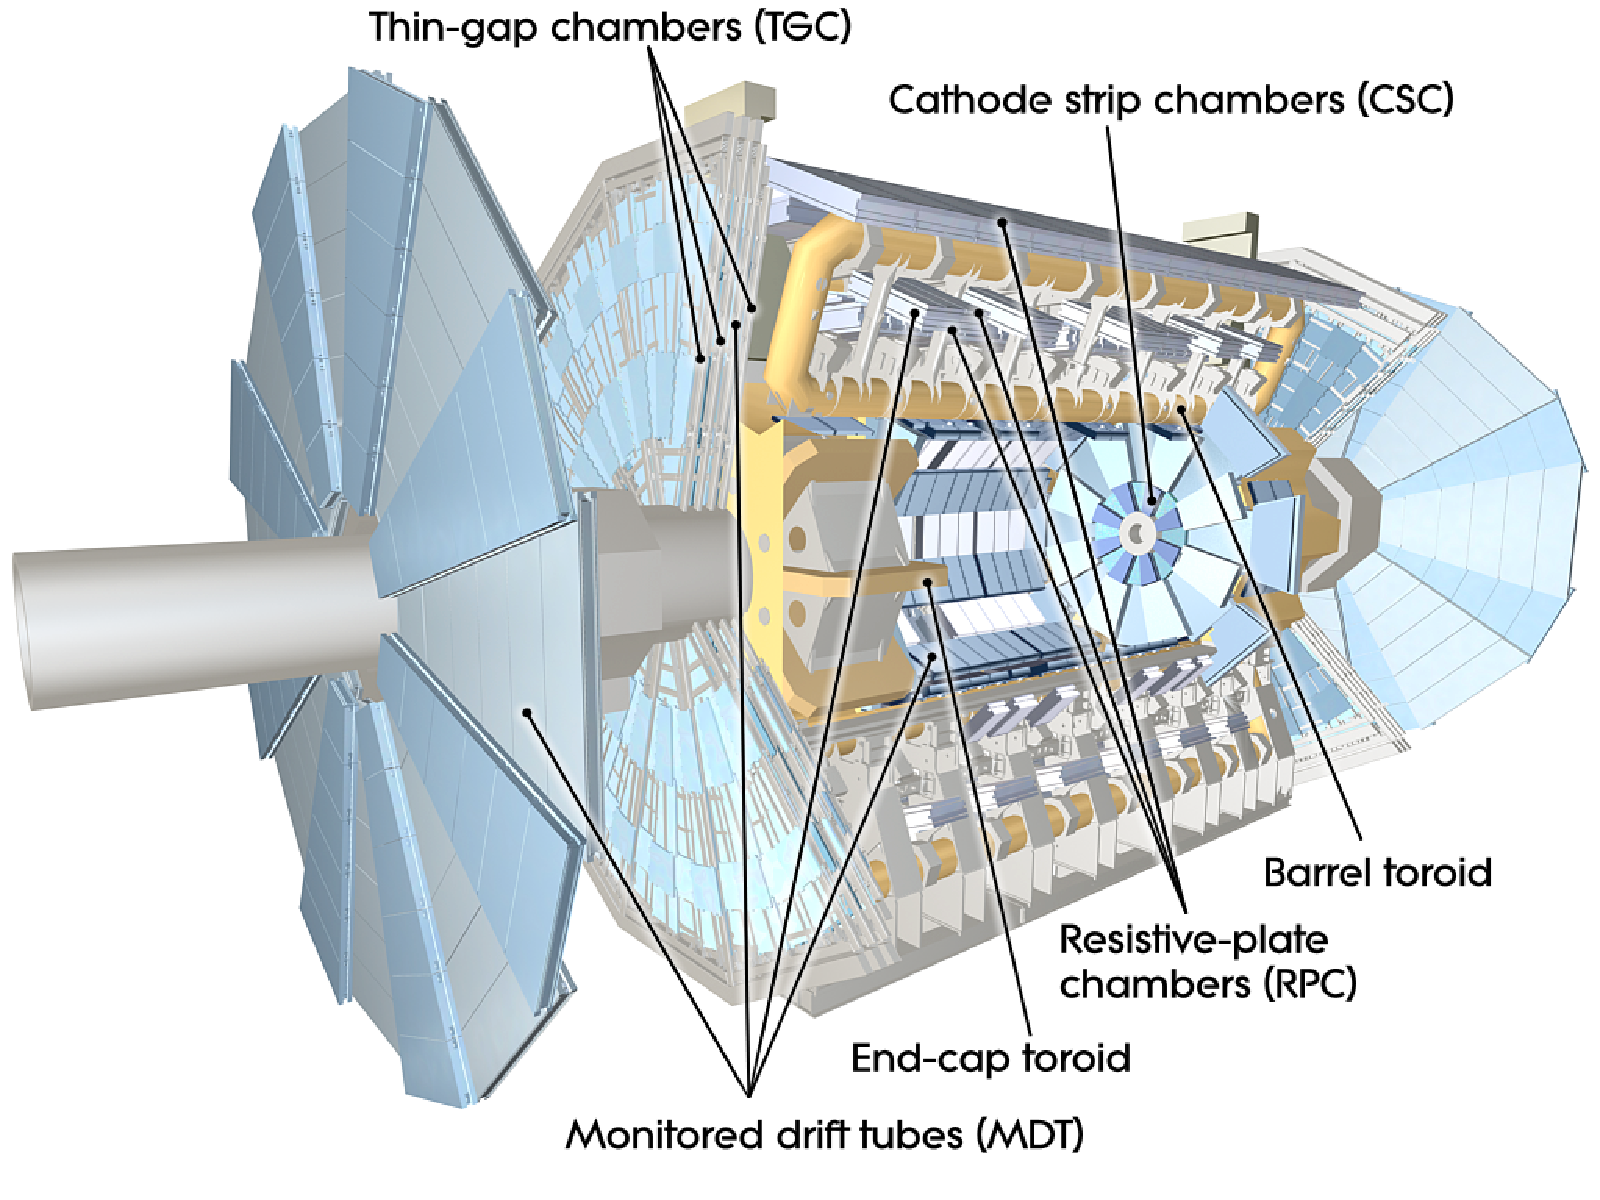
\includegraphics[width=\hsize]{figures/Detector/muonsys.pdf}
  \caption{Schematic of Muon Spectrometer [cite G35]} 
  \label{fig:muonsys}
\end{figure}
\FloatBarrier


\begin{figure}[h!]
  \centering
  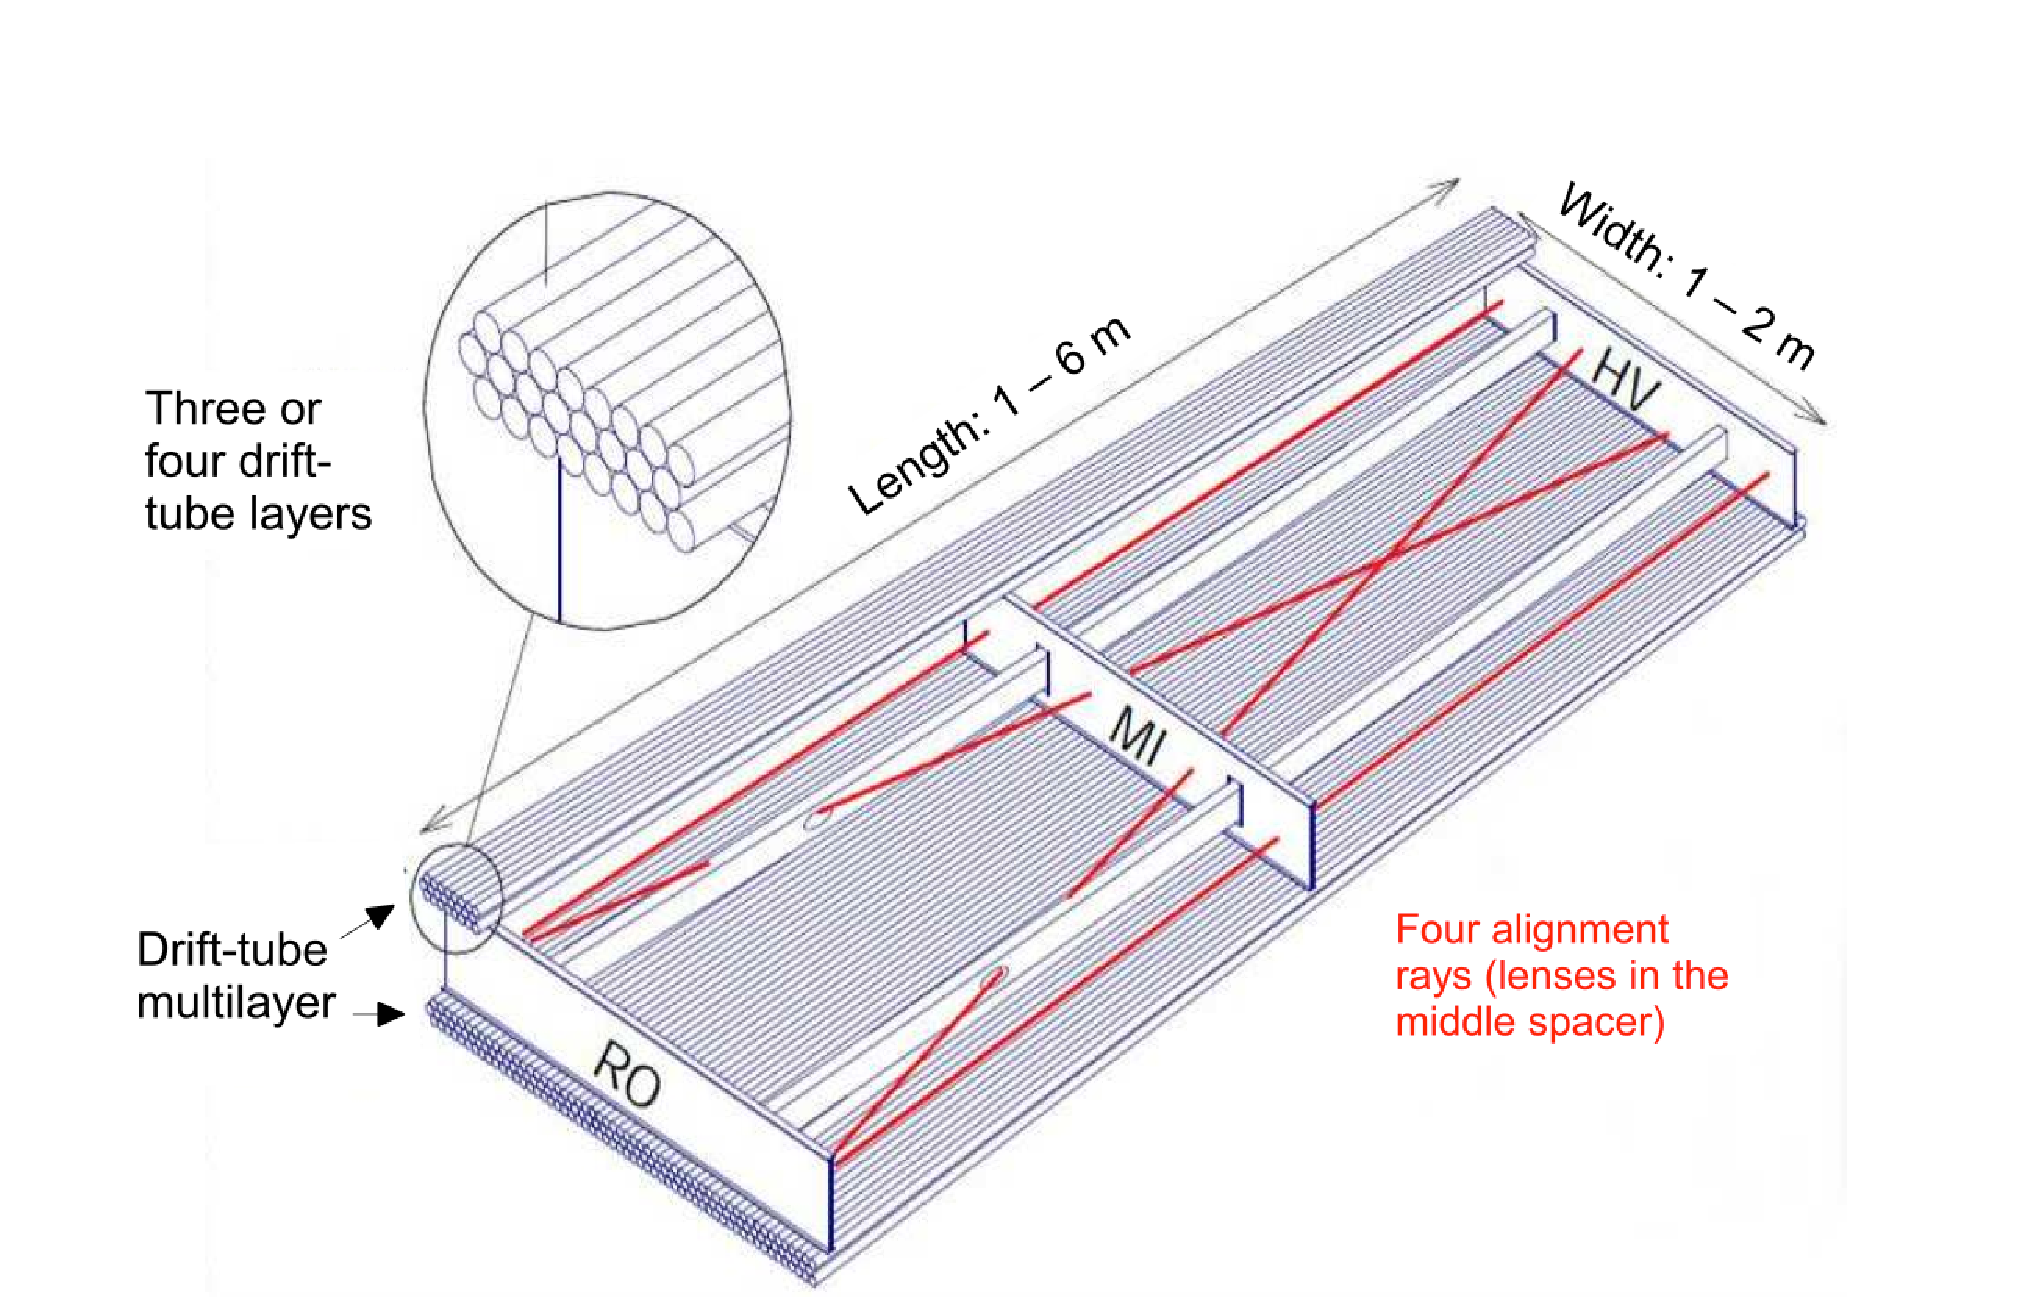
\includegraphics[width=\hsize]{figures/Detector/muon_mdt.pdf}
  \caption{Schematic of MDT chamber. [cite G35]} 
  \label{fig:muon_mdt}
\end{figure}
\FloatBarrier


\begin{figure}[h!]
  \centering
  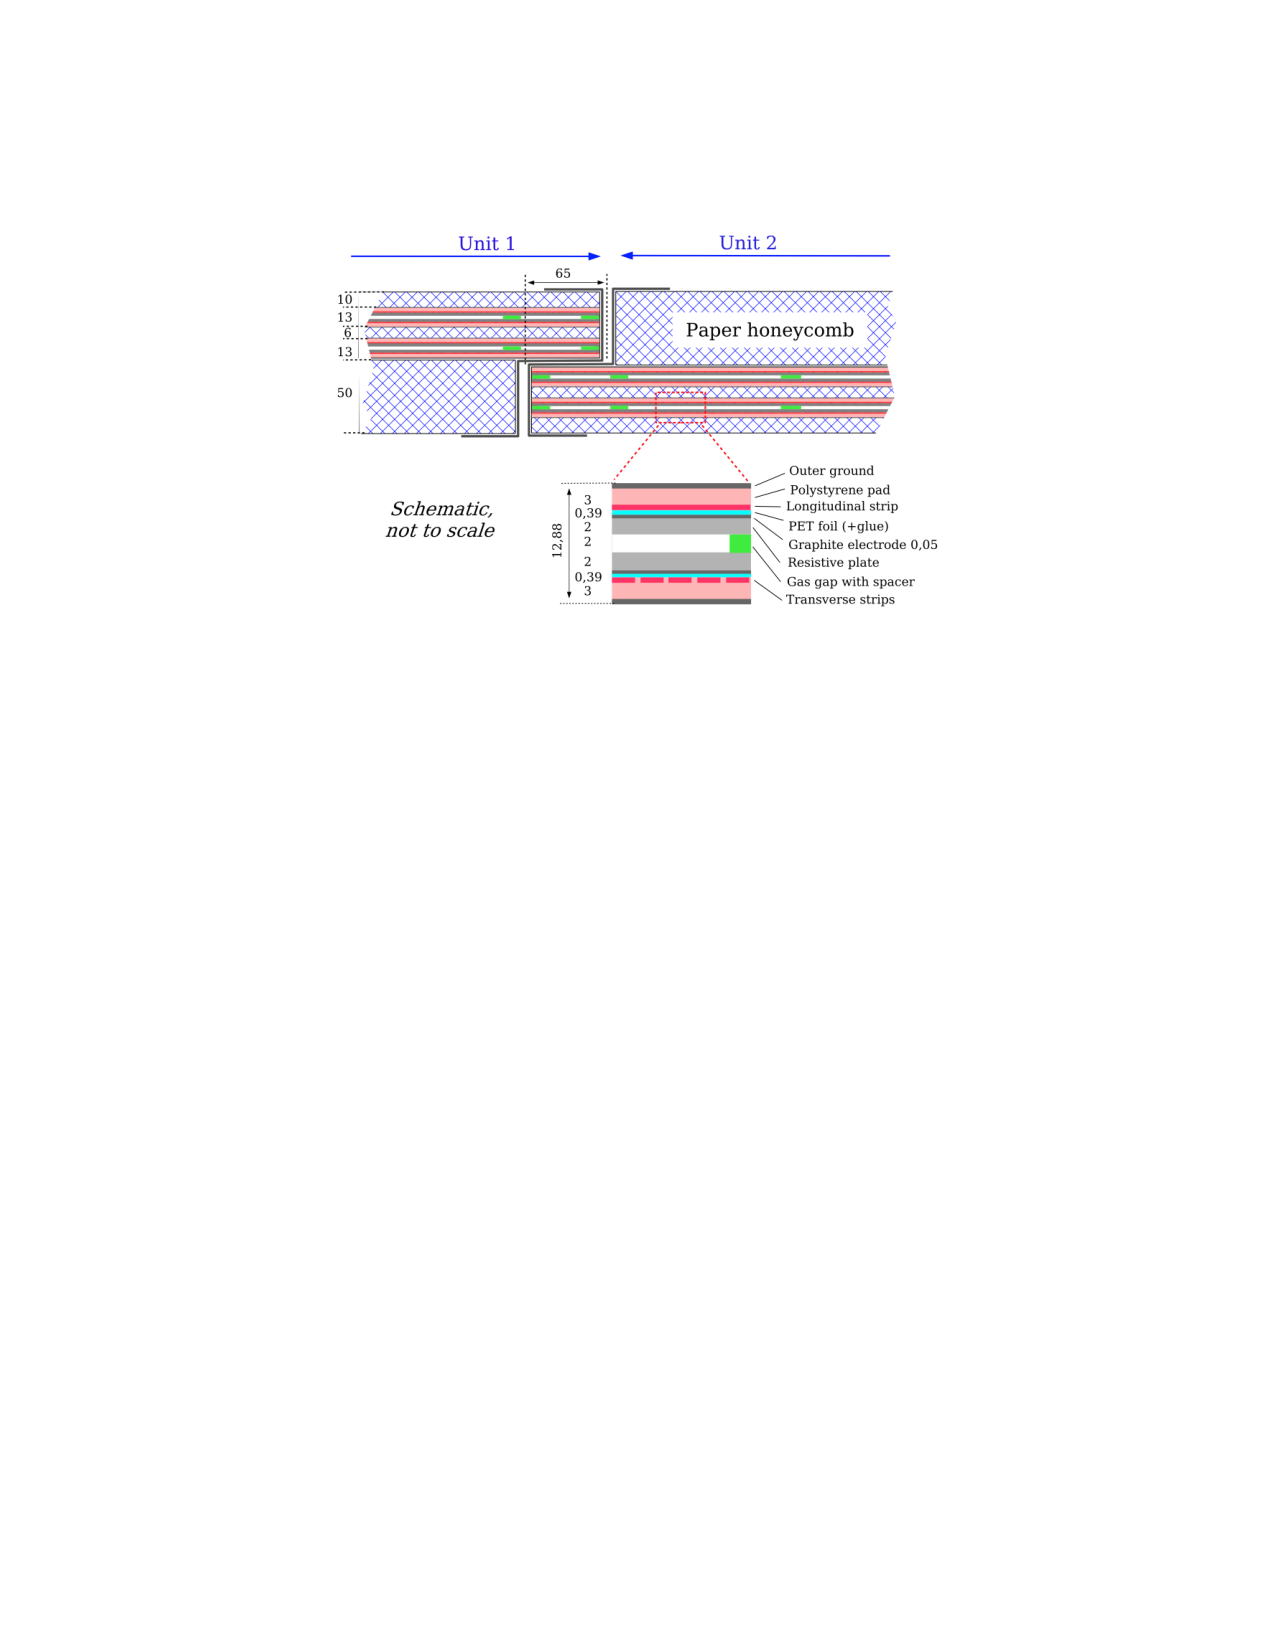
\includegraphics[width=\hsize]{figures/Detector/muon_rpc.pdf}
  \caption{Schematic of RPC chamber, which is used for triggering in the central region of the detector [cite G35].} 
  \label{fig:muon_rpc}
\end{figure}
\FloatBarrier



\begin{figure}[h!]
  \centering
  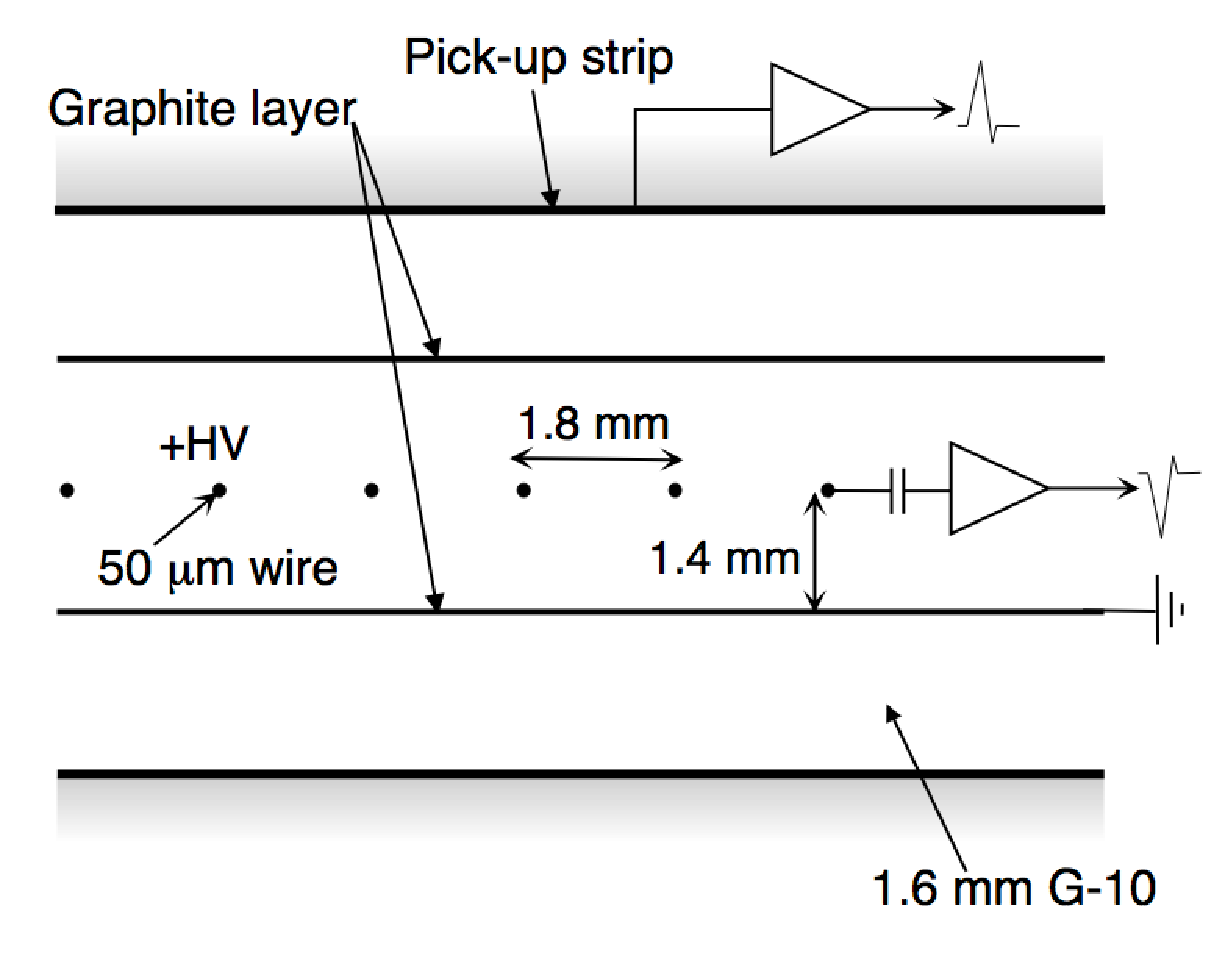
\includegraphics[width=\hsize]{figures/Detector/muon_tgc.pdf}
  \caption{Schematic of TGC chamber, which is used for triggering in the muon end-cap region. [cite G35]} 
  \label{fig:muon_tgc}
\end{figure}
\FloatBarrier

\section{Magnet System}
A particles with charge, q, and velocity v, moving in magnetic field, B, experiences a force, $F= qv\times B$. This force can cause charged particles to have a curved trajectory in magnetic fields, which the ID and MS use to determine the particles $p_{T}$. The central solenoid provides the magnetic field for the ID and the toroidal magnets provide the magnetic field for the MS.

The layout of the magnet system is shown in Figure \ref{fig:atlas_magnets}. The central solenoid consists of a single-layer Al-stabilized NbTi conductor coil wound inside an Al support cylinder. The solenoid is 5.8 m long, 50 cm thick and has an inner radius of 1.23 m. It is cooled to 4.5 K to reach superconducting temperatures and shares the liquid argon calorimeter vacuum vessel to minimize material in the detector. A current of 7.730kA produces a 1.998 T solenodial magnetic field, pointing in the +$z$ direction. 

The toroidal magnet system consists of a barrel and two end-cap toroidal magnets used to create a magnetic field outside the calorimeters that is orientated along $\phi$. Each barrel toroid is 25.3 m long with an inner and outer diameter of 9.4 and 20.1 m and weighs 830 tonnes. Endcap toroids are 5 m long with an inner and outer radius of 1.65 and 10.7 m. Both toroid systems use Al-stabilized Nb/Ti/Cu conductors. The magnetic field strength in the barrel and endcap regions are 0.5 and 1 T, respectively.

\begin{figure}[h!]
  \centering
  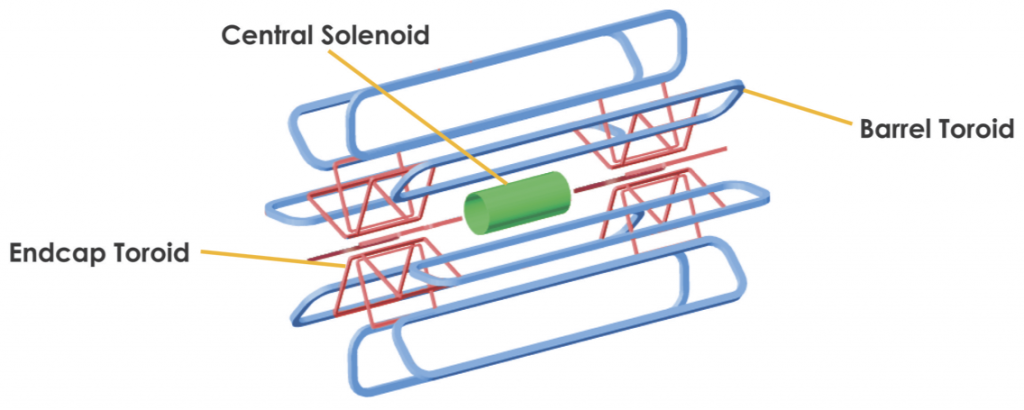
\includegraphics[width=\hsize]{figures/Detector/atlas_magnets.png}
  \caption{Layout of ATLAS magnet systems.} 
  \label{fig:atlas_magnets}
\end{figure}
\FloatBarrier


\section{Trigger System}
Since collisions occur every 25 ns and reading out all detector channels and storing that information is not currently feasible (would require saving 60 million megabytes per second), the majority of events are not kept for analysis. ATLAS uses a multi-stage trigger system to select approximately 1,000 of the 1.7 billion collisions that occur each second (corresponding to a rate of 1 kHz from the 40 MHz proton collision rate). The first stage of the trigger system is the hardware level (L1) trigger. This trigger reduces the event rate to $\sim$100 kHz by identifying Regions-of-Interest (ROIs) containing high $p_{T}$ leptons, photons, jets, or $E_{T}^{miss}$ by using information from RPCs, TGCs, and calorimeters to make a 2.5 $\mu$s decision. This information is then passed to a high-level trigger (HLT) which further decreases event rates to $\sim$ 1 kHz. The HLT uses finer granularity measurements from the MS and ID to preform simplified offline reconstruction to decide which events to keep.
